\paragraph{QuizziPedia::Front-End::Views::ConnectionQuestionsView}
\begin{figure} [ht]
	\centering
	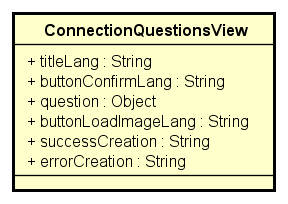
\includegraphics[scale=0.80]{UML/Classi/Front-End/QuizziPedia_Front-end_Views_ConnectionQuestionsView.png}
	\caption{QuizziPedia::Front-End::Views::ConnectionQuestionsView}
\end{figure} \FloatBarrier
\begin{itemize}
	\item \textbf{Descrizione}: view contenente i campi e le direttive per creare una domanda a collegamento;
	\item \textbf{Utilizzo}: permette all'utente di creare una domanda a collegamento compilando i campi proposti;
	\item \textbf{Relazioni con altre classi}:
	\begin{itemize}
		\item \textit{IN} \texttt{ConnectionQuestionsModelView}: classe di tipo modelview la cui istanziazione è contenuta all'interno della variabile di ambiente \$scope di \texttt{Angular.js}. All'interno di essa sono presenti le variabili e i metodi necessari per il \textit{Two-Way Data-Binding\ped{G}} tra la view \texttt{ConnectionQuestionsView} e il controller \texttt{ConnectionQuestionsController};
		\item \textit{IN} \texttt{InputToListModelView}: classe di tipo modelview la cui istanziazione è contenuta all'interno della variabile di ambiente \$scope di \texttt{Angular.js}. All'interno di essa sono presenti le variabili e i metodi necessari per il \textit{Two-Way Data-Binding\ped{G}} tra la view \texttt{ConnectionQuestionsView} e il controller \texttt{InputToListController};
		\item \textit{IN} \texttt{TopicKeywordsDirective}: directive che permette di gestire l'inserimento di keywords al momento della creazione della domanda;
		\item \textit{IN} \texttt{QuestionTextDirective}: rappresenta il componente grafico che permette all'utente di scrivere o modificare il testo di una domanda;
		\item \textit{IN} \texttt{LangModel}: rappresenta il modello delle informazioni per la giusta traduzione dell'applicazione.
	\end{itemize}
	\item \textbf{Attributi}:
	\begin{itemize}
		\item \texttt{+ question: Object} \\ Oggetto contenente gli attributi per la creazione della domanda:
		\begin{itemize}
			\item \texttt{answer}: array contenente oggetti che rappresentano le risposte. Ogni oggetto risposta contiene:
			\begin{itemize}
				\item \texttt{text1}: di tipo \texttt{String}, rappresenta il primo elemento testuale che sarà collegato ad un secondo elemento (testuale o immagine);
				\item \texttt{text2}:  di tipo \texttt{String}, rappresenta il secondo elemento testuale che sarà collegato al primo elemento (testuale o immagine);
				\item \texttt{url1}: di tipo \texttt{String}, rappresenta il primo elemento immagine che sarà collegato con il secondo elemento (testuale o immagine);
				\item \texttt{url2}: di tipo \texttt{String}, rappresenta il secondo elemento immagine che sarà collegato con il primo elemento (testuale o immagine).
			\end{itemize}
		\end{itemize}			
		\item \texttt{+ titleLangConnection: String} \\ Attributo che viene utilizzato per visualizzare la giusta traduzione del titolo della pagina, in italiano o in inglese;
		\item \texttt{+ buttonConfirmLangConnection: String} \\ Attributo che viene utilizzato per visualizzare la giusta traduzione della \textit{label\ped{G}} per il bottone di conferma, in italiano o in inglese;
		\item \texttt{+ buttonLoadImageLangConnection: String} \\ Attributo che viene utilizzato per visualizzare la giusta traduzione della \textit{label\ped{G}} per il bottone di caricamento dell'immagine nel testo della domanda, in italiano o in inglese;
		\item \texttt{+ successCreation: String} \\ Attributo che visualizza un messaggio di conferma avvenuta creazione della domanda;
		\item \texttt{+ errorCreation: String} \\ Attributo che visualizza un messaggio d'errore per la creazione della domanda.
	\end{itemize}
\end{itemize}